% !TeX root = RJwrapper.tex
\title{Hyper-Poisson Regression Modeling via GAMLSS}


\author{by Freddy Hernández-Barajas, Jamiu S. Olumoh, Osho O. Ajayi, and Fernando Marmolejo-Ramos}

\maketitle

\abstract{%
Traditional Poisson regression assumes equal mean and variance, which is often violated in practice. Hyper-Poisson regression addresses this by accommodating under-dispersed and over-dispersed data. The proposed DiscreteDists R package integrates the hyper-Poisson distribution functions into the GAMLSS framework, enabling more accurate count data analysis. This study examines the capabilities of the DiscreteDists R package, which includes functions for both parameterizations of the hyper-Poisson distribution and its regression model. This paper demonstrates the implementation of hyper-Poisson regression using the DiscreteDists R package, offering enhanced tools for researchers. In addition, the study includes simulation studies and practical applications to demonstrate the performance and utility of the proposed R package.
}

\section{Introduction}\label{introduction}

The conventional Poisson regression assumes that the mean and variance of the count data are equal; however, this assumption is often violated in practice. The hyper-Poisson regression proposed by \citet{Saez13} is a recent statistical modeling technique used to analyze count data where the variance is less than or greater than the mean. In many real-world scenarios, count data with under-dispersion (variance \(<\) mean) or over-dispersion (variance \(>\) mean) is common, and numerous examples abound in the fields of epidemiology, ecology, education, and finance, among others \citet{Cameron1988Microeconomics}, \citet{Consul1989}, \citet{Winkelmann1991}, \citet{Famoye1993}, \citet{johnson2005}, \citet{Sellers2012}.

Generalized additive models for location, scale, and shape (GAMLSS) is a flexible regression framework that can handle a wide range of data distributions, including count data with under-dispersion or over-dispersion \citet{Stasinopoulos2008}. GAMLSS is an extension of the generalized linear model (GLM) that allows for simultaneously modeling the mean, variance, skewness, and kurtosis of the response variable. This makes GAMLSS particularly useful for modeling complex data that exhibit non-standard patterns of variation \citet{peluso2019discrete}.

In GAMLSS, the response variable is modeled using a set of additive predictor functions, each of which corresponds to different aspects or properties of the response variable. These quantities include the location (usually the mean or median), scale (usually the standard deviation or precision), and shape (such as skewness and kurtosis) parameters \citet{Marmolejo-Ramos2023}. These predictor functions are typically constructed using smoothing functions that include splines and/or kernel smoothers because of their flexibility in describing the relationships between the response and predictor variable(s) \citet{elbachir2018}.

The hyper-Poisson distribution was initially proposed by \citet{BardwellCrow1964}. The first parameterization of the distribution has two parameters (\(\lambda\) for location and \(\gamma\) for dispersion), but neither of these parameters coincides with the distribution's mean value. For this reason, the authors presented a second parameterization of the hyper-Poisson distribution, also with two parameters (\(\mu\) for location and \(\gamma\) for dispersion). In this new parameterization, the expected value coincides with the location parameter \(\mu\), making it attractive for creating a regression model to analyze real datasets. If one parameter matches the expected value, the regression model is appealing to any user due to the interpretability of this parameter.

\citet{Saez13} proposed the hyper-Poisson regression model and \citet{DGLMExtPois_pack} proposed the \CRANpkg{DGLMExtPois} R package to fit the hyper-Poisson regression model. This package includes useful functions for estimating the effect of covariates on the parameters of the hyper-Poisson regression model (modeling \(\mu\) and \(\gamma\)). Additionally, this package contains functions for the COM regression model \citet{huang2017} to perform residual analysis. Unfortunately, the \CRANpkg{DGLMExtPois} R package lacks the basic functions to calculate probabilities and quantiles and generate random values for both parameterizations of the hyper-Poisson distribution.

In this paper, we describe the capabilities of our proposed \CRANpkg{DiscreteDists} R package, which includes functions for both parameterizations of the hyper-Poisson distribution and the regression model. Our implementation is integrated within the GAMLSS framework, allowing us to model both distribution parameters using covariates. By using the \CRANpkg{DiscreteDists} R package \citet{DiscreteDists_pack}, researchers can perform hyper-Poisson regression analyses more accurately and efficiently, enhancing their ability to uncover meaningful insights from count data with under-dispersion or over-dispersion.

The remaining parts of this paper are organized as follows: Section 2 presents the hyper-Poisson distribution and the regression model based on the second parameterization. Section 3 explains the GAMLSS statistical framework. Section 4 introduces the main functions of the \CRANpkg{DiscreteDists} R package. Section 5 presents the results of a simulation study to explore the performance of the proposed functions to estimate parameters, and Section 6 presents applications of the hyper-Poisson regression model to a real dataset. Finally, Section 7 presents the conclusions of the paper.

\section{The hyper-poisson model}\label{the-hyper-poisson-model}

The attraction of the hyper-Poisson model is its ability to effectively capture the behavior of a count data set that is either under-dispersed or over-dispersed, or that satisfies the equality of the mean and variance as the basic Poisson distribution.

\subsection{The hyper-Poisson distribution}\label{the-hyper-poisson-distribution}

The hyper-Poisson distribution was proposed by \citet{BardwellCrow1964}, and it is appropriate for over-dispersed, equi-dispersed, or under-dispersed discrete count data \(Y\). Its mass function with location \(\mu\) and dispersion \(\sigma\) parameters is given by:

\begin{equation} 
    f(y | \mu, \sigma) = \frac{\mu^y}{_1F_1(1;\sigma;\mu)}\frac{\Gamma(\sigma)}{\Gamma(\sigma + y)}, \;\;\;\; y=0,1,2, 3, \ldots; \mu>0; \sigma>0
  \label{eq:pdfhp}
\end{equation}

This distribution is over-dispersed when \(\sigma > 1\), under-dispersed when \(\sigma<1\), and equi-dispersed (i.e.~Poisson) when \(\sigma = 1\). The function \(_1F_1\) is defined as:

\begin{equation}
    _1F_1(a;c;z) = \sum_{r=0}^{\infty}\frac{(a)_r}{(c)_r}\frac{z^r}{r!},
  \label{eq:1f1p}
\end{equation}

with \((a)_r = \frac{\Gamma(a+r)}{\Gamma(a)}\) for real values \(a>0\) and \(r\) a positive integer. In particular, \(_1F_1(1;c, z)\) is the confluent hypergeometric function with the first argument equal to unity.

To denote that a random variable \(Y\) follows the hyper-Poisson distribution with parameters \(\mu\) and \(\sigma\) we will use the notation \(Y \sim HYPERPO(\mu, \sigma)\). Figure \ref{fig:pmf} depicts an example of the probabilities for the \(HYPERPO(\mu=5.5, \sigma)\) and three possible values of the second parameter, \(\sigma=0.1\) (under-dispersed), \(\sigma=1.0\) (Poisson or equi-dispersed) and \(\sigma=1.9\) (over-dispersed).

\begin{figure}
\includegraphics[width=0.8\linewidth,height=0.32\textheight]{RJ-2026-004_files/figure-latex/pmf-1} \caption{Probability mass function for the HYPERPO with three different values for the second parameter.}\label{fig:pmf}
\end{figure}

Equation \eqref{eq:pdfhp} is known to satisfy the recurrence relation:

\begin{equation} 
(y + \mu)f_{y + 1} = \sigma f_y,
  \label{eq:rec-rel}
\end{equation}

which when summed over all values of the random variable \(Y\), yields expressions \(E(Y)\) for the mean and \(V(Y)\) for the variance of the distribution:

\begin{equation} 
E(Y) = \mu - (\sigma-1) \frac{_1F_1(1;\sigma;\mu)-1}{_1F_1(1;\sigma;\mu)}
  \label{eq:mean}
\end{equation}

\begin{equation} 
V(Y) = \mu + \left[ \mu-(\sigma-1) \right] E(Y) - E^2(Y)
  \label{eq:var}
\end{equation}

In the equations above, \(E(Y)\) is a function of parameters \(\mu\) and \(\sigma\), whereas \(V(Y)\) is a function of \(\mu\), \(\sigma\) and \(E(Y)\). When the dispersion parameter \(\sigma = 1\) (i.e., the equi-dispersion case), then clearly \(E(Y) = \mu\) in equation \eqref{eq:mean} and hence the location parameter coincides with the theoretical expectation of a Poisson distribution assumption for the dataset. Using the same argument in equation \eqref{eq:mean} and setting \(\sigma < 1\) leads to under-dispersion, while setting \(\sigma > 1\) means over-dispersion.

The probability mass function for the hyper-Poisson distribution has been written here with parameters \(\mu\) and \(\sigma\) and not using \(\lambda\) and \(\gamma\) as in \citet{BardwellCrow1964} and \citet{Saez13}; this was done mainly because those are the Greek letters used in the GAMLSS framework.

In the statistical literature, several traditional distributions (both continuous and discrete) have been reparameterized so that one of their parameters coincides with the expected value. For example, \citet{rigby2019distributions} (p.~84) introduced the distribution WEI3, a reparameterization of the Weibull distribution in which the first parameter \(\mu\) corresponds to the mean. A discrete case can be found in \citet{ribeiro2020reparametrization}, where the authors proposed a new parameterization of the Conway--Maxwell--Poisson distribution to ensure that the first parameter represents the mean.

Following this idea, \citet{Saez13} proposed reexpressing the original HYPERPO distribution in the parameterization HYPERPO2, in which the first parameter \(\mu\) coincides with the expected value. The approach is based on expression \eqref{eq:mean}, substituting \(\mu\) by \(\lambda\), and then, for a given \(E(Y)\) and \(\sigma\), solving for \(\lambda\) in the equation.

\begin{equation} 
E(Y) = \lambda - (\sigma-1) \frac{_1F_1(1;\sigma;\lambda)-1}{_1F_1(1;\sigma;\lambda)}.
  \label{eq:isolatelambda}
\end{equation}

Because \(\lambda\) appears inside the confluent hypergeometric function \(_1F_1\), it cannot be isolated in a closed form, and must therefore be obtained numerically. Consequently, a closed expression for the PDF is not available.

\begin{table}[h] \centering 
\caption{Comparative table between the two parametrizations of the hyper-Poisson distribution. The $\lambda$ value in HYPERPO2 is obtained from the expression (6) given $E(Y)$ and $\sigma$.} \label{tab:placeholder} 
\begin{tabular}{cccc} \hline 
Param. & pdf & $E(Y)$ & $Var(Y)$ \\ \hline 
HYPERPO & Expression (1) & $\mu - (\sigma-1) \frac{_1F_1(1;\sigma;\mu)-1}{_1F_1(1;\sigma;\mu)}$ & $\mu + \left[ \mu-(\sigma-1) \right] E(Y) - E^2(Y)$ \\ 
HYPERPO2 & Not available & $\mu$ & $\lambda + \left[ \lambda-(\sigma-1) \right] \mu - \mu^2$ \\ \hline 
\end{tabular} 
\end{table}

As noted in \citet{Saez13}, solving for \(\lambda\) in \eqref{eq:isolatelambda} represents a computational challenge during parameter estimation, since \(\lambda\) must be computed numerically at each evaluation of the log-likelihood.

\subsection{The hyper-Poisson regression model}\label{the-hyper-poisson-regression-model}

\citet{Saez13} extended the model of \citet{BardwellCrow1964} to the situation in which the response variable \(Y\) is explained using the explanatory variables \(X_1, X_2, \ldots, X_p\). In this situation, \(y_i\) represents the observed value of \(Y\) and \(x_{i1}, x_{i2}, x_{i3}, \dots, x_{ip}\) represents the observed values of the explanatory variables (with \(i=1, 2, \ldots, n\)). The approach proposed by \citet{Saez13} models the mean \(\mu\) of \(Y\) and the dispersion parameter \(\sigma\), rather than the canonical parameter \(\lambda\). For this reason, we refer to this as the second parameterization of the hyper-Poisson distribution. The hyper-Poisson regression model under this parameterization can be expressed as:

\begin{equation} 
\mu_i = \exp(\boldsymbol{W}_i \boldsymbol{\beta}),
  \label{eq:mu}
\end{equation}

\begin{equation} 
\sigma_i = \exp(\boldsymbol{Z}_i \boldsymbol{\delta}).
  \label{eq:sig}
\end{equation}

The vectors \(\boldsymbol{W}_i\) and \(\boldsymbol{Z}_i\) are subsets of the explanatory variables \(X_1, X_2, \ldots, X_p\) and the vectors \(\boldsymbol{\beta}\) and \(\boldsymbol{\delta}\) are the effects vectors for the explanatory variables related to \(\mu\) and \(\sigma\), respectively. Given this definition, the model \(hP(\mu_i(\boldsymbol{\beta}), \, \sigma_i(\boldsymbol{\delta}))\) now becomes a function of the parameters \(\boldsymbol{\beta}\) and \(\boldsymbol{\delta}\). These parameters are estimated using the maximum likelihood approach.

\section{Generalized additive models for location, scale, and shape (GAMLSS)}\label{generalized-additive-models-for-location-scale-and-shape-gamlss}

Generalized Additive Models for Location, Scale, and Shape (GAMLSS) is a statistical framework that extends traditional generalized linear models (GLMs) to accommodate a wide range of response distributions, including non-Gaussian and heteroscedastic data \citep{Rigby2005}. Within GAMLSS, the assumption of an exponential family distribution for the dependent (response) variable is relaxed and substituted with a general distribution family, which includes highly skewed and/or kurtosis, continuous and discrete distributions \citep{Rigby2005, Stasinopoulos2008}. GAMLSS expands the systematic component of the model, enabling the modeling not only of the location measure (such as mean, median, or mode) but also other parameters of the distribution of the dependent variable as linear and/or non-linear, parametric, and/or additive non-parametric functions of explanatory variables and/or random effects. Consequently, GAMLSS is particularly well-suited for modeling response variables that do not follow an exponential family distribution \citep{Stasinopoulos2008, Marmolejo-Ramos2022}. This includes variables with characteristics such as leptokurtic or platykurtic distributions, positive or negative skewness, over-dispersed counts, or heterogeneity where the scale or shape of the distribution of the dependent variable changes with explanatory variable(s). Thus, GAMLSS enables modeling the relationships between predictors (covariates) and a response variable while also accounting for the distributional characteristics of the response variable. This makes GAMLSS a powerful tool for handling complex and diverse data types.

\subsection{Model Frame}\label{model-frame}

Consider a location regression model that establishes a relationship between a dependent (response) variable and one or more explanatory variables, defined by \citet{Nelder1972} as the general form of the Generalized Linear Model

\begin{equation}
g(\mu) = X \beta 
\label{eq:glm}
\end{equation}

where \(Y\) represents the response variable, \(\mu\) denotes the expected value of \(Y\), \(X\) is the matrix of predictor/explanatory variables (also known as the design matrix), \(\beta\) represents the vector of coefficients, and \(g\) is the link function. Equation \eqref{eq:glm} relates the linear predictor \(X \beta\) to the expected value \(\mu\) of the response variable through the link function \(g\). The specific form of the link function and the choice of probability distribution for \(Y\) depend on the type of GLM used. The relationship between \(\mu\) and \(X \beta\) can be expressed using the inverse link function:

\begin{equation}
\mu = g^{-1}(X \beta) 
\label{eq:ginv}
\end{equation}

When other statistical measures, such as variance, skewness, and kurtosis, are influenced by explanatory variables, the Generalized Additive Models for Location, Scale, and Shape (GAMLSS) framework becomes a plausible alternative to extend beyond mean regression models \citep[\citet{Ramires2021}]{Kneib2013}. This extension generalizes both the concepts of Generalized Linear Models \citep{Nelder1972} and Generalized Additive Models \citep{Hastie1990}.

GAMLSS, a class of semi-parametric regression models, is designed to describe the response variable \(Y\) while accommodating diverse regression structures to explain any or all of its parameters using linear and/or nonlinear functions \citep{Rigby2005}. Assuming that \(Y\) follows a distribution \(D(\theta)\) with a probability density function as described in equation \eqref{eq:pdfhp}, and \(\theta\) is its parameter vector associated with the explanatory variables, GAMLSS can be formulated as a function of regressors:

\begin{equation}
 g_k (\theta_k) = \eta_k = X_k \beta_k + \sum_{j=1}^{J_k} s_{jk} (x_{jk}) 
  \label{eq:gamless}
\end{equation}

Here, \(g_k(\cdot)\) refers to a suitable link function for the \(k\)-th parameter, generally determined by the parameter range considered \citep{Stasinopoulos2017}. \(X_{k}\) is a known fixed \(n \times (m_{k} + 1)\) model matrix, \(m_{k}\) denotes the number of explanatory variables related to the \(k\)-th parameter, \(\beta_{k} = (\beta_{0k}, \beta_{1k}, \dots, \beta_{m_{k}k})^T\) represents a parameter vector of length \((m_{k} +1)\), and \(s_{jk}(\cdot)\) denotes smoothing functions that depend on variable \(X_{jk}\), that is, \(s_{jk} (x_{jk})\) is a vector that evaluates function \(s_{jk}\) at \(x_{jk}\), the quantity \(J_k\) represents the number of explanatory variables \(X\) passed to the \(k\)-th parameter by the smoothing function. If the additive term \(\sum_{j=1}^{J_k} s_{jk} (x_{jk}) = 0\) then, equation \eqref{eq:gamless} reduces to parametric form. Furthermore, various additive terms like cubic splines, penalized splines, fractional polynomials, LOESS curves, ridge, principal component regression (PCR), simple random effects, varying coefficient, neural networks, kernels, regression trees, and LASSO and elastic net, etc, can be employed to address nonlinearity, structural changes, and other data peculiarities \citep{gamlss.book.2024}.

Implementation of GAMLSS is available in R through packages such as \CRANpkg{gamlss}, \CRANpkg{gamlss.data}, and \CRANpkg{gamlss.dist}, among others; these packages provide (penalized) likelihood-fitting algorithms, datasets, and distributions, respectively. Additionally, other packages can work in conjunction with GAMLSS; those packages are: the \CRANpkg{gamboostLSS} package by \citet{gamboostLSS_pack} implements boosting methods for GAMLSS models, while the \CRANpkg{bamlss} package by \citet{bamlss_pack} fits a GAMLSS model to data using the protocol of Bayesian MCMC. GAMLSS can also connect with machine learning techniques like neural networks, regression trees \CRANpkg{pcr}, semi-structured distributional regression \citep{SSDR.2024}, and the Grammar of Graphics \CRANpkg{ggplot2}.

\subsection{Likelihood and link}\label{likelihood-and-link}

Suppose that we have a dataset consisting of observations \(y_{1}, y_{2}, ..., y_{n}\) that is assumed to come from the hyper-Poisson distribution. The likelihood function \(L(\mu, \sigma | y)\) for this data is the probability of observing the given data under the distribution in equation \eqref{eq:pdfhp}. The product of the individual PMF values for each observation is given as:

\begin{equation}    
L(\mu, \sigma | y) = \prod_{i=1}^{n} \frac{\mu ^{y_{i}}}{_1F_1(1;\mu;\sigma)}\frac{\Gamma(\sigma)}{\Gamma(y_{i}+ \sigma)}.
\label{eq:lik}
\end{equation}

To maximise the likelihood function and estimate the parameters \(\mu\) and \(\sigma\), we defined the log-likelihood function as:

\begin{equation}
\log L(\mu,\sigma | y) = \sum_{i=1}^{n} \left[ y_i \log(\mu) - \log\left({_1F_1(1;\mu;\sigma)}\right) + \log\left(\frac{\Gamma(\sigma)}{\Gamma(y_i+ \sigma)}\right) \right].
\label{eq:logli}
\end{equation}

\section{Implementation of the hyper-poisson distribution in R}\label{implementation-of-the-hyper-poisson-distribution-in-r}

The \CRANpkg{DiscreteDists} package implements the hyper-Poisson distribution within a GAMLSS framework. This package allows users to estimate the parameters for the distribution or estimate the effects of the regression model. The current version of the package is available on CRAN, and users can download it using the following code.

\begin{verbatim}
install.packages("DiscreteDists")
library(DiscreteDists)
\end{verbatim}

In the \CRANpkg{DiscreteDists} package, we implemented two parameterizations of the hyper-Poisson distribution:

\begin{itemize}
\tightlist
\item
  \texttt{HYPERPO(mu,\ sigma)}: this parameterization corresponds to the original proposal given in expression \eqref{eq:pdfhp}. The location parameter is \(\mu>0\), and the scale parameter \(\sigma>0\). In this parameterization the \(E(Y)\) is a function of both parameters \(\mu\) and \(\sigma\), it is \(E(Y)=\mu-(\sigma-1)(1-1/_1F_1(1;\sigma;\mu))\).
\item
  \texttt{HYPERPO2(mu,\ sigma)}: this second parameterization represents an alternative parameterization. The location parameter is \(\mu>0\), and the scale parameter \(\sigma>0\). This parameterization is attractive because \(E(Y)=\mu\), the expected value coincides with the location parameter \(\mu\).
\end{itemize}

In practice, users can use both parameterizations, \texttt{HYPERPO(mu,\ sigma)} or \texttt{HYPERPO2(mu,\ sigma)}. The advantage of using the second parameterization is that the parameter \(\mu\) coincides with the expected value \(E(Y)\) of the response variable.

The \CRANpkg{DiscreteDists} package provides the usual functions to calculate probabilities, cumulative probabilities, quantiles, and generate random samples. Table 2 summarizes the functions available for each parameterization of the hyper-Poisson distribution. The main functions to estimate parameters within the GAMLSS framework are \texttt{HYPERPO} and \texttt{HYPERPO2}. Since the expected value and variance for the hyper-Poisson distribution do not have closed forms, the functions \texttt{mean\_var\_hp} and \texttt{mean\_var\_hp2} allow obtaining those values for both parametrizations. Additionally, Table 2 shows the related functions in the \CRANpkg{DGLMExtPois} under each parametrization.

\begin{table}[h]
\caption{Functions for the hyper-Poisson distribution in DiscreteDists and DGLMExtPois under two parametrizations.}\label{table:funcs}
\begin{tabular}{ccccc} \hline 
Package   & \multicolumn{2}{c}{\CRANpkg{DiscreteDists}} & \multicolumn{2}{c}{\CRANpkg{DGLMExtPois}} \\ \hline
Function               & First param. & Second param. & First param. & Second param \\ \hline
Probability            &  \code{dHYPERPO} & \code{dHYPERPO2} & \code{dhP} & -- \\
Cumulative             &  \code{pHYPERPO} & \code{pHYPERPO2} & \code{phP} & -- \\
Quantile               &  \code{qHYPERPO} & \code{qHYPERPO2} & --  & -- \\
Random                 &  \code{rHYPERPO} & \code{rHYPERPO2} & \code{rhP} & -- \\
Mean-variance          &  \code{mean\_var\_hp} & \code{mean\_var\_hp2} & -- & -- \\
Estimation parameters  &  \code{HYPERPO}  & \code{HYPERPO2}  & -- & \code{glm\_CMP} \\ \hline 
\end{tabular}
\end{table}

The proposed \CRANpkg{DiscreteDists} R package integrates smoothly with the existing gamlss ecosystem of packages, such as \CRANpkg{gamlss}, \CRANpkg{gamlss.dist}, \CRANpkg{gamlss.cens}, \CRANpkg{bamlss}, among others. This ensures that both implementations of the hyper-Poisson distribution provided in the package can be used in the traditional way within the ecosystem by all users.

\subsection{Examples for the first parameterization}\label{examples-for-the-first-parameterization}

This section provides examples of using the package functions for the first parameterization HYPERPO. Suppose we want to obtain probabilities for \(HYPERPO(\mu=5.5, \sigma=0.1)\) when \(y=0, 1, \ldots, 10\). To do this, we can use the following code:

\begin{verbatim}
library(DiscreteDists)
dHYPERPO(x=0:10, mu=5.5, sigma=0.1)
\end{verbatim}

\begin{verbatim}
#>  [1] 9.262073e-05 5.094140e-03 2.547070e-02 6.670898e-02 1.183546e-01
#>  [6] 1.587684e-01 1.712208e-01 1.543795e-01 1.195897e-01 8.120290e-02
#> [11] 4.907867e-02
\end{verbatim}

As mentioned, the hyper-Poisson distribution with \(\sigma=1\) coincides with the Poisson distribution. We can check this by comparing the results from \(HYPERPO(\mu=5.5, \sigma=1)\) with \(Poisson(\lambda=5.5)\) as follows:

\begin{verbatim}
dHYPERPO(x=0:10, mu=5.5, sigma=1)
\end{verbatim}

\begin{verbatim}
#>  [1] 0.004086771 0.022477243 0.061812418 0.113322766 0.155818804 0.171400684
#>  [7] 0.157117294 0.123449302 0.084871395 0.051865853 0.028526219
\end{verbatim}

\begin{verbatim}
dpois(x=0:10, lambda=5.5)
\end{verbatim}

\begin{verbatim}
#>  [1] 0.004086771 0.022477243 0.061812418 0.113322766 0.155818804 0.171400684
#>  [7] 0.157117294 0.123449302 0.084871395 0.051865853 0.028526219
\end{verbatim}

Additionally to the \texttt{dHYPERPO} function, the \CRANpkg{DiscreteDists} package contains the \texttt{pHYPERPO} function to obtain cumulative probabilities, \texttt{qHYPERPO} to obtain quantiles, and \texttt{rHYPERPO} to generate random values of the hyper-Poisson distributions. Below we present an example of how to simulate 500 values from \(HYPERPO(\mu=5.5, \sigma=0.1)\).

\begin{verbatim}
set.seed(1234)
y <- rHYPERPO(n=500, mu=5.5, sigma=0.1)
y[1:15]
\end{verbatim}

\begin{verbatim}
#>  [1]  4  7  7  7  9  7  2  5  7  6  7  6  5 10  5
\end{verbatim}

We can explore the empirical mean and variance from the \texttt{y} vector as follows:

\begin{verbatim}
mean(y)
\end{verbatim}

\begin{verbatim}
#> [1] 6.478
\end{verbatim}

\begin{verbatim}
var(y)
\end{verbatim}

\begin{verbatim}
#> [1] 5.672862
\end{verbatim}

The \CRANpkg{DiscreteDists} package contains the function \texttt{mean\_var\_hp}, useful for obtaining the theoretical mean and variance for \(HYPERPO(\mu, \sigma)\) using the expressions \eqref{eq:mean} and \eqref{eq:var}. In the following, we can find the R code to obtain the theoretical mean and variance for \(HYPERPO(\mu=5.5, \sigma=0.1)\). We observe that the empirical mean and variance are close to the theoretical values.

\begin{verbatim}
mean_var_hp(mu=5.5, sigma=0.1)
\end{verbatim}

\begin{verbatim}
#> $mean
#> [1] 6.399917
#> 
#> $variance
#> [1] 5.500533
\end{verbatim}

Recall that in the first parameterization of the hyper-Poisson distribution, the parameter \(\mu\) is not the expected value \(E(Y)\), for this reason, in this example \(E(Y)=6.399917\) whereas \(\mu=5.5\).

The \CRANpkg{DiscreteDists} package contains the \texttt{HYPERPO} function family, which allows for estimating parameters via the GAMLSS framework. Below we can find the R code to estimate \(\mu\) and \(\sigma\) parameters using the \texttt{y} vector.

\begin{verbatim}
library(gamlss)
mod1 <- gamlss(y ~ 1, family=HYPERPO)
\end{verbatim}

\begin{verbatim}
#> GAMLSS-RS iteration 1: Global Deviance = 2261.591
\end{verbatim}

\begin{verbatim}
summary(mod1)
\end{verbatim}

\begin{verbatim}
#> ******************************************************************
#> Family:  c("HYPERPO", "Hyper-Poisson") 
#> 
#> Call:  gamlss(formula = y ~ 1, family = HYPERPO) 
#> 
#> Fitting method: RS() 
#> 
#> ------------------------------------------------------------------
#> Mu link function:  log
#> Mu Coefficients:
#>             Estimate Std. Error t value Pr(>|t|)    
#> (Intercept)  1.71244    0.05607   30.54   <2e-16 ***
#> ---
#> Signif. codes:  0 '***' 0.001 '**' 0.01 '*' 0.05 '.' 0.1 ' ' 1
#> 
#> ------------------------------------------------------------------
#> Sigma link function:  log
#> Sigma Coefficients:
#>             Estimate Std. Error t value Pr(>|t|)
#> (Intercept)   -2.748      4.559  -0.603    0.547
#> 
#> ------------------------------------------------------------------
#> No. of observations in the fit:  500 
#> Degrees of Freedom for the fit:  2
#>       Residual Deg. of Freedom:  498 
#>                       at cycle:  1 
#>  
#> Global Deviance:     2261.591 
#>             AIC:     2265.591 
#>             SBC:     2274.021 
#> ******************************************************************
\end{verbatim}

From the last output we can find that \(\hat{\mu}=\exp(1.71244)=5.542469\) and \(\hat{\sigma}=\exp(-2.748)=0.06405584\), estimates that are close to the true values \(\mu=5.5\) and \(\sigma=0.1\).

In this last example, we simulate a dataset for the hyper-Poisson regression model with a response variable \(Y\) and two covariates \(X_1\) and \(X_2\). The model to generate the dataset is given below.

\begin{equation}
    \begin{split}
        y_i &\sim HYPERPO(\mu _i, \sigma_i), \\
        \log(\mu_i) &= 1.21 - 3 \times X_{1i}, \\
        \log(\sigma_i) &= 1.26 - 2\times X_{2i},\\
        X_1 &\sim U(0, 1), \\
        X_2 &\sim U(0, 1).
    \end{split}
\label{eq:example3}
\end{equation}

In the following code, we are going to simulate 200 observations of the model and then we estimate the vector parameter \(\boldsymbol{\Theta}=(1.21, -3, 1.26, -2)^\top\) using the \texttt{HYPERPO} function family taking advantage of the GAMLSS framework.

\begin{verbatim}
# A function to simulate a data set with Y ~ HYPERPO2
gendat <- function(n) {
  x1 <- runif(n)
  x2 <- runif(n)
  mu    <- exp(1.21 - 3 * x1)
  sigma <- exp(1.26 - 2 * x2)
  y <- rHYPERPO(n=n, mu=mu, sigma=sigma)
  data.frame(y=y, x1=x1, x2=x2)
}

set.seed(1234)
dataset <- gendat(n=200)

mod2 <- gamlss(y~x1, sigma.fo=~x2, family=HYPERPO, 
               control=gamlss.control(n.cyc=50, trace=FALSE),
               data=dataset)
\end{verbatim}

Using the \texttt{summary} function, we can obtain a summary table with the usual information for a GAMLSS model.

\begin{verbatim}
summary(mod2)
\end{verbatim}

\begin{verbatim}
#> ******************************************************************
#> Family:  c("HYPERPO", "Hyper-Poisson") 
#> 
#> Call:  gamlss(formula = y ~ x1, sigma.formula = ~x2, family = HYPERPO,  
#>     data = dataset, control = gamlss.control(n.cyc = 50, trace = FALSE)) 
#> 
#> Fitting method: RS() 
#> 
#> ------------------------------------------------------------------
#> Mu link function:  log
#> Mu Coefficients:
#>             Estimate Std. Error t value Pr(>|t|)    
#> (Intercept)   1.0775     0.1255   8.587 2.62e-15 ***
#> x1           -2.5758     0.2935  -8.775 7.93e-16 ***
#> ---
#> Signif. codes:  0 '***' 0.001 '**' 0.01 '*' 0.05 '.' 0.1 ' ' 1
#> 
#> ------------------------------------------------------------------
#> Sigma link function:  log
#> Sigma Coefficients:
#>             Estimate Std. Error t value Pr(>|t|)    
#> (Intercept)   1.0599     0.2295   4.619 6.94e-06 ***
#> x2           -2.0979     0.4559  -4.601 7.49e-06 ***
#> ---
#> Signif. codes:  0 '***' 0.001 '**' 0.01 '*' 0.05 '.' 0.1 ' ' 1
#> 
#> ------------------------------------------------------------------
#> No. of observations in the fit:  200 
#> Degrees of Freedom for the fit:  4
#>       Residual Deg. of Freedom:  196 
#>                       at cycle:  45 
#>  
#> Global Deviance:     471.7851 
#>             AIC:     479.7851 
#>             SBC:     492.9784 
#> ******************************************************************
\end{verbatim}

From the last summary we observe that \(\hat{\boldsymbol{\Theta}}=(1.0775, -2.5758, 1.0599, -2.0979)^\top\) while the true parameter vector is \(\boldsymbol{\Theta}=(1.21, -3, 1.26, -2)^\top\).

Since the examples for the second parameterization (HYPERPO2) follow the same structure as those already presented, they are omitted for brevity.

\section{Simulation study}\label{simulation-study}

In this section, we showcase the outcomes of a Monte Carlo simulation study that examines parameter estimation for models with and without covariates under the second parameterization (HYPERPO2). To assess the effectiveness of estimating a general parameter \(\theta\), we employed the mean value and the Mean Squared Error \((MSE)\) of the estimator \(\hat{\theta}\). Those metrics are defined as follows:

\begin{align*} 
    \text{Mean value} &= \frac{\sum_{i=1}^{i=k}{\hat{\theta}_i}}{k}  \\ 
    \text{Mean Squared Error}  &= \frac{\sum_{i=1}^{i=k}{(\hat{\theta}_i - \theta)^2}}{k}
\end{align*}

\subsection{Model without covariates}\label{model-without-covariates}

During the first part of the simulation study, we utilized data generated from a \(HYPERPO2(\mu, \sigma)\) distribution. The model employed for this segment can be succinctly summarized as follows:

\begin{equation}
    \begin{split}
        y_i    &\sim HYPERPO2(\mu, \sigma), \\
        \mu    &\in \{3, 7\}, \\
        \sigma &\in \{0.5, 1, 1.5\}.
    \end{split}
\label{eq:model1}
\end{equation}

For each value of sample size \(n=50, 100, 200, \ldots, 1000\), we followed the next steps to simulate the data and estimate the parameters:

\begin{itemize}
\tightlist
\item
  Generate a sample of size \(n\) from a \(HYPERPO2(\mu, \sigma)\).
\item
  Obtain and store the estimations \(\hat{\mu}\) and \(\hat{\sigma}\) using the proposed procedure.
\item
  Repeat steps 1 to 2 \(k=1,000\) times.
\end{itemize}

\subsection{Model with covariates}\label{model-with-covariates}

In the second part of the simulation study, we considered data generated from the next model:

\begin{equation}
    \begin{split}
        y_i &\sim HYPERPO2(\mu _i, \sigma_i), \\
        \log(\mu_i) &= \beta_0 + \beta_1 \times X_{1i} + \beta_2 \times X_{11i}, \\
        \log(\sigma_i) &= \gamma_0 + \gamma_1 \times X_{2i} + \gamma_2 \times X_{22i},\\
        X_1 &\sim U(0, 1), \\
        X_{11} &\sim U(0, 1), \\
        X_2 &\sim U(0, 1), \\
        X_{22} &\sim U(0, 1).
    \end{split}
\label{eq:model2}
\end{equation}

The parameter vector was fixed as \(\boldsymbol{\theta}=(\beta_0=1.21, \beta_1=-3.0, \beta_2=2.0, \gamma_0=1.26, \gamma_1=-2.0, \gamma_2=1.5)^\top\). From model \eqref{eq:model2}, we have that \(X_1 \sim U(0, 1)\) and \(X_11 \sim U(0, 1)\), it implies that \(\mu \approx \exp(1.21 - 3.0 \times 0.5 + 2.0 \times 0.5) = 2.03\). The same analysis can be done for the \(\sigma\) parameter to obtain \(\sigma \approx 2.75\).

For each value of sample size \(n=50, 100, 200, \ldots, 1000\), we followed the next steps to simulate the data and estimate the parameters:

\begin{itemize}
\tightlist
\item
  Generate a random sample of \(n\) values from a \(HYPERPO2\) distribution given in expression \eqref{eq:model2}.
\item
  Obtain and store the estimations \(\hat{\beta}_0\), \(\hat{\beta}_1\), \(\hat{\gamma}_0\) and \(\hat{\gamma}_1\) using the proposed procedure.
\item
  Repeat steps 1 to 2 for \(k=1,000\) times.
\end{itemize}

All scripts used in the simulation study are available as supplementary material in a GitHub repository at \url{https://github.com/fhernanb/HYPERPO_paper}.

\subsection{Results for the simulations without covariates}\label{results-for-the-simulations-without-covariates}

Figures \ref{fig:case1mu3} and \ref{fig:case1mu7} depict the mean values of the estimated parameters \(\hat{\mu}\) and \(\hat{\sigma}\) plotted against the sample size \(n\) for several combinations of \(\mu\) and \(\sigma\). A general pattern observed is that as the sample size increases, the estimated parameters tend towards the true values, indicated by the horizontal red lines.

\begin{figure}

{\centering 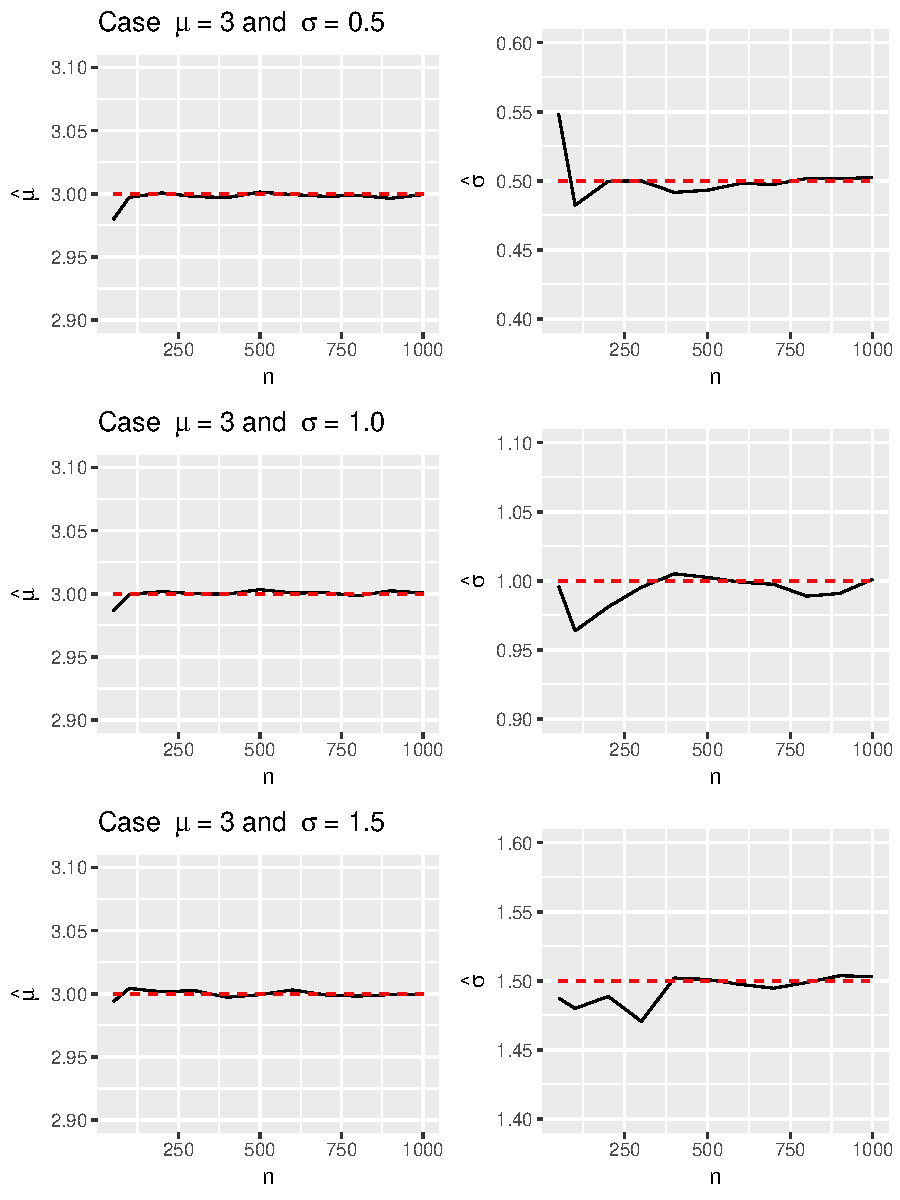
\includegraphics[width=0.5\linewidth,height=0.4\textheight,alt={}]{figures/case1_mean_true_mu=3} 

}

\caption{Mean for the estimated parameters $\hat{\mu}$ (on left) and $\hat{\sigma}$ (on right) versus $n$ for $\mu=3$ and $\sigma=0.5, 1.0, 1.5$. Red horizontal lines correspond to the true values of $\mu$ and $\sigma$.}\label{fig:case1mu3}
\end{figure}

\begin{figure}

{\centering 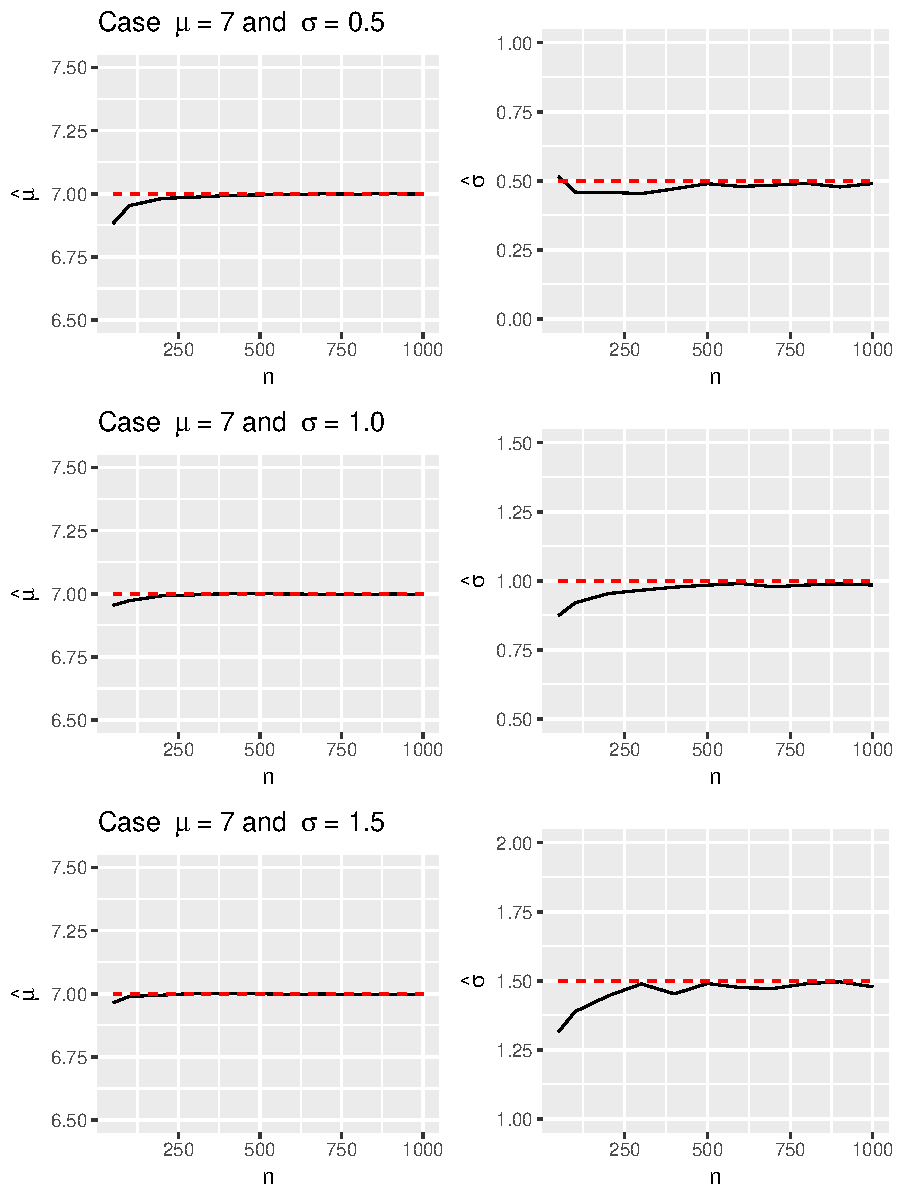
\includegraphics[width=0.5\linewidth,height=0.4\textheight,alt={}]{figures/case1_mean_true_mu=7} 

}

\caption{Mean for the estimated parameters $\hat{\mu}$ (on left) and $\hat{\sigma}$ (on right) versus $n$ for $\mu=7$ and $\sigma=0.5, 1.0, 1.5$. Red horizontal lines correspond to the true values of $\mu$ and $\sigma$.}\label{fig:case1mu7}
\end{figure}

Figures \ref{fig:case1mse3} and \ref{fig:case1mse7} depict the Mean Squared Error (MSE) of the estimated parameters \(\hat{\mu}\) and \(\hat{\sigma}\) plotted against the sample size \(n\) for various combinations of \(\mu\) and \(\sigma\). A consistent trend observed is that with an increase in the sample size, the MSE converges toward zero, as expected.

\begin{figure}

{\centering 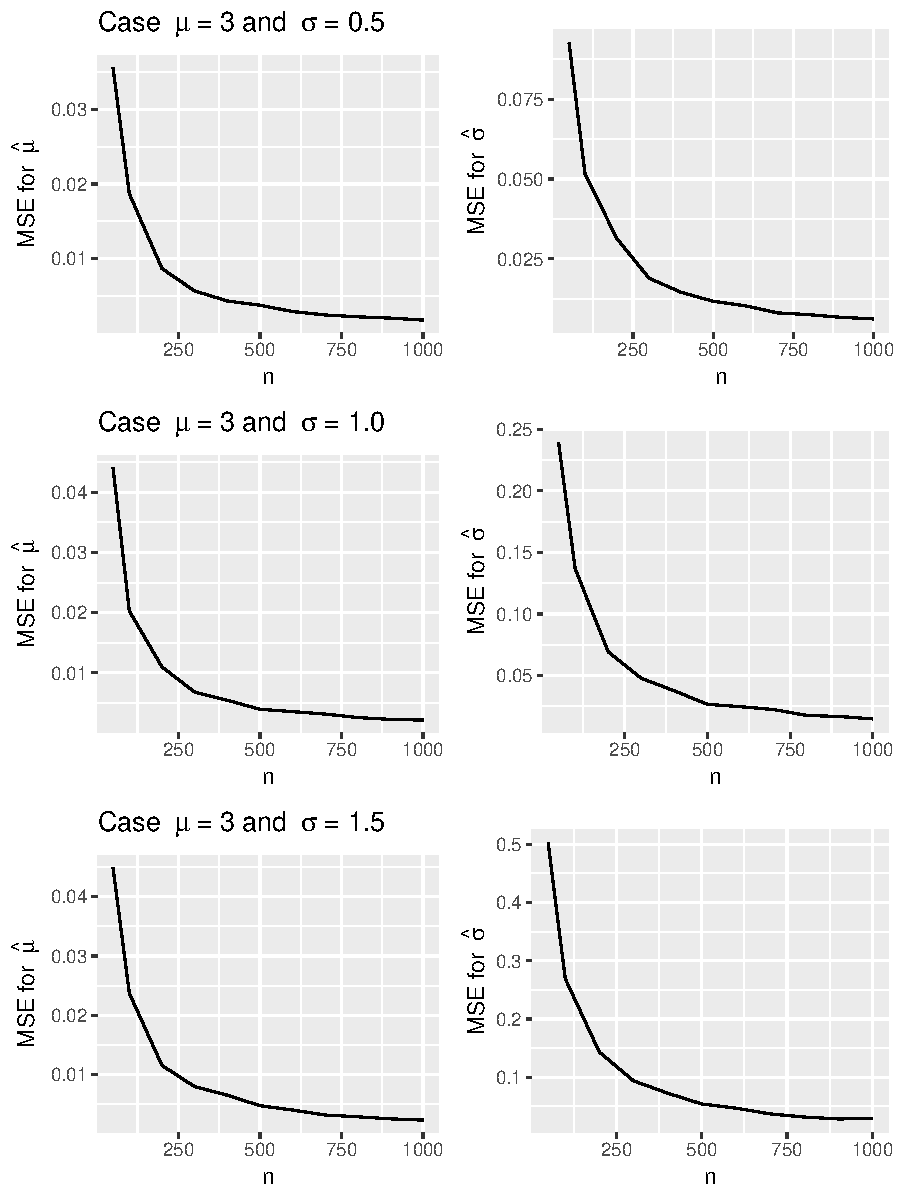
\includegraphics[width=0.5\linewidth,height=0.4\textheight,alt={}]{figures/case1_mse_true_mu=3} 

}

\caption{MSE for the estimated parameters $\hat{\mu}$ (on left) and $\hat{\sigma}$ (on right) versus $n$ for $\mu=3$ and $\sigma=0.5, 1.0, 1.5$. Red horizontal lines correspond to the true values of $\mu$ and $\sigma$.}\label{fig:case1mse3}
\end{figure}

\begin{figure}

{\centering 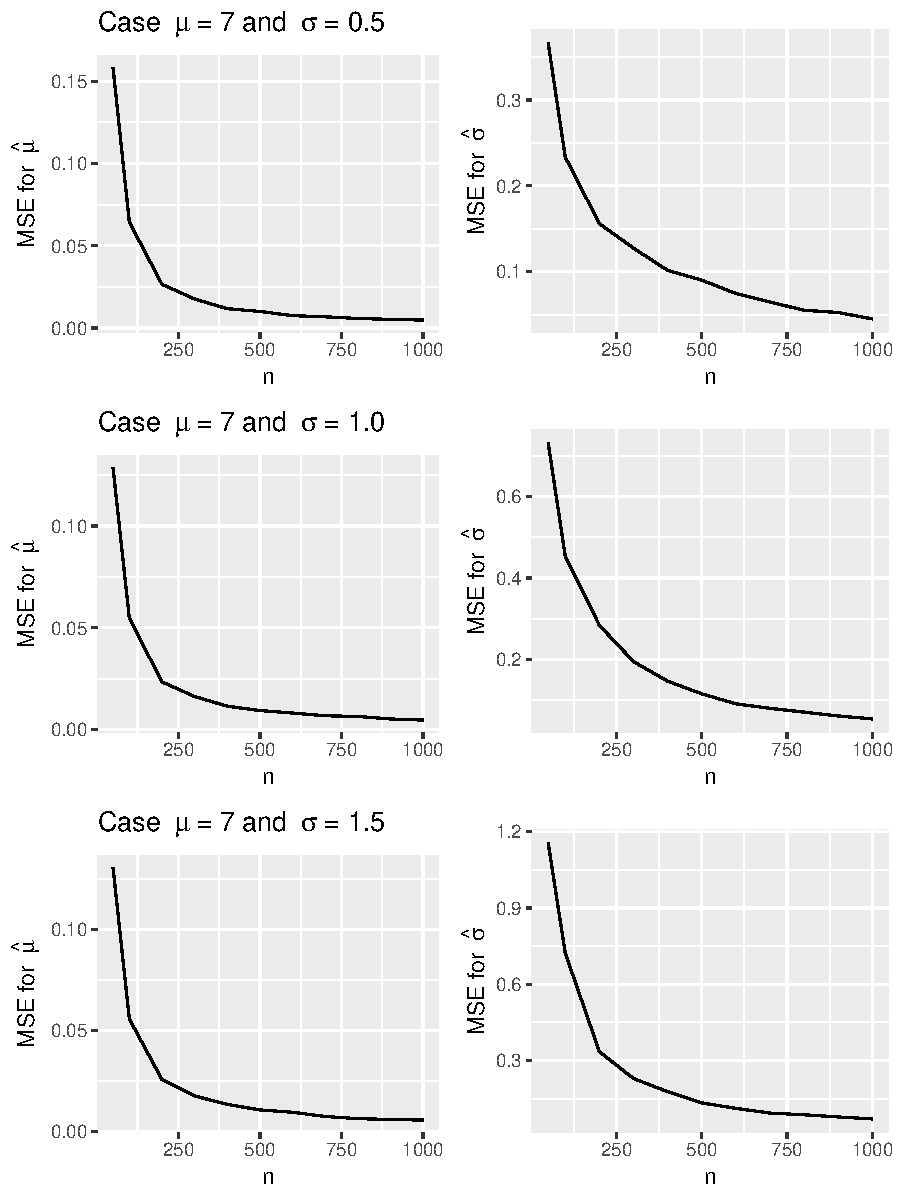
\includegraphics[width=0.5\linewidth,height=0.4\textheight,alt={}]{figures/case1_mse_true_mu=7} 

}

\caption{MSE for the estimated parameters $\hat{\mu}$ (on left) and $\hat{\sigma}$ (on right) versus $n$ for $\mu=7$ and $\sigma=0.5, 1.0, 1.5$. Red horizontal lines correspond to the true values of $\mu$ and $\sigma$.}\label{fig:case1mse7}
\end{figure}

\subsection{Results for the simulations with covariates}\label{results-for-the-simulations-with-covariates}

Figures \ref{fig:case2mean} and \ref{fig:case2mse} illustrate the mean values and Mean Squared Error (MSE) of the estimated parameters \(\hat{\beta}_0\), \(\hat{\beta}_1\), \(\hat{\beta}_2\) \(\hat{\gamma}_0\), \(\hat{\gamma}_1\) and \(\hat{\gamma}_2\) plotted against the sample size \(n\). A prevailing trend observed is that with an increase in the sample size, the estimated parameters converge towards the true values, denoted by the horizontal red lines, while the MSE approaches zero.

\begin{figure}

{\centering 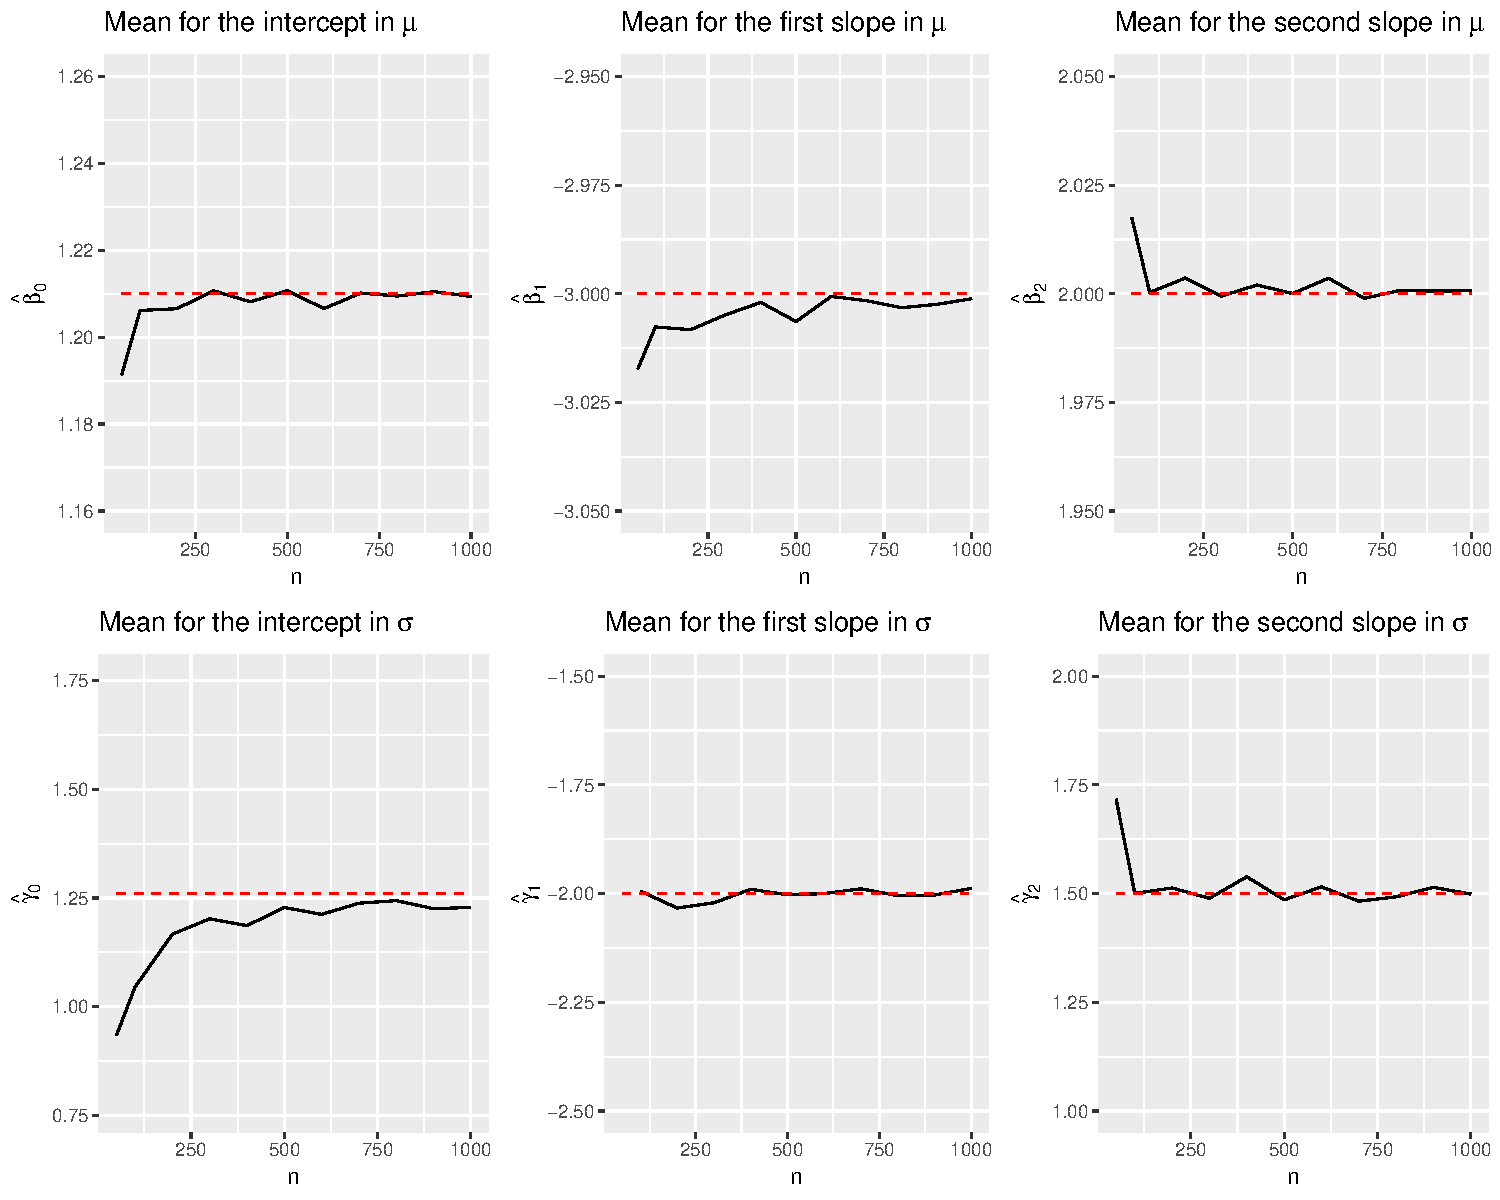
\includegraphics[width=0.6\linewidth,height=0.3\textheight,alt={}]{figures/case2_mean} 

}

\caption{Mean for the estimated parameters $\hat{\beta}_0$, $\hat{\beta}_1$, $\hat{\beta}_2$, $\hat{\gamma}_0$, $\hat{\gamma}_1$ and $\hat{\gamma}_2$ versus $n$. Red horizontal lines correspond to the objective value.}\label{fig:case2mean}
\end{figure}

\begin{figure}

{\centering 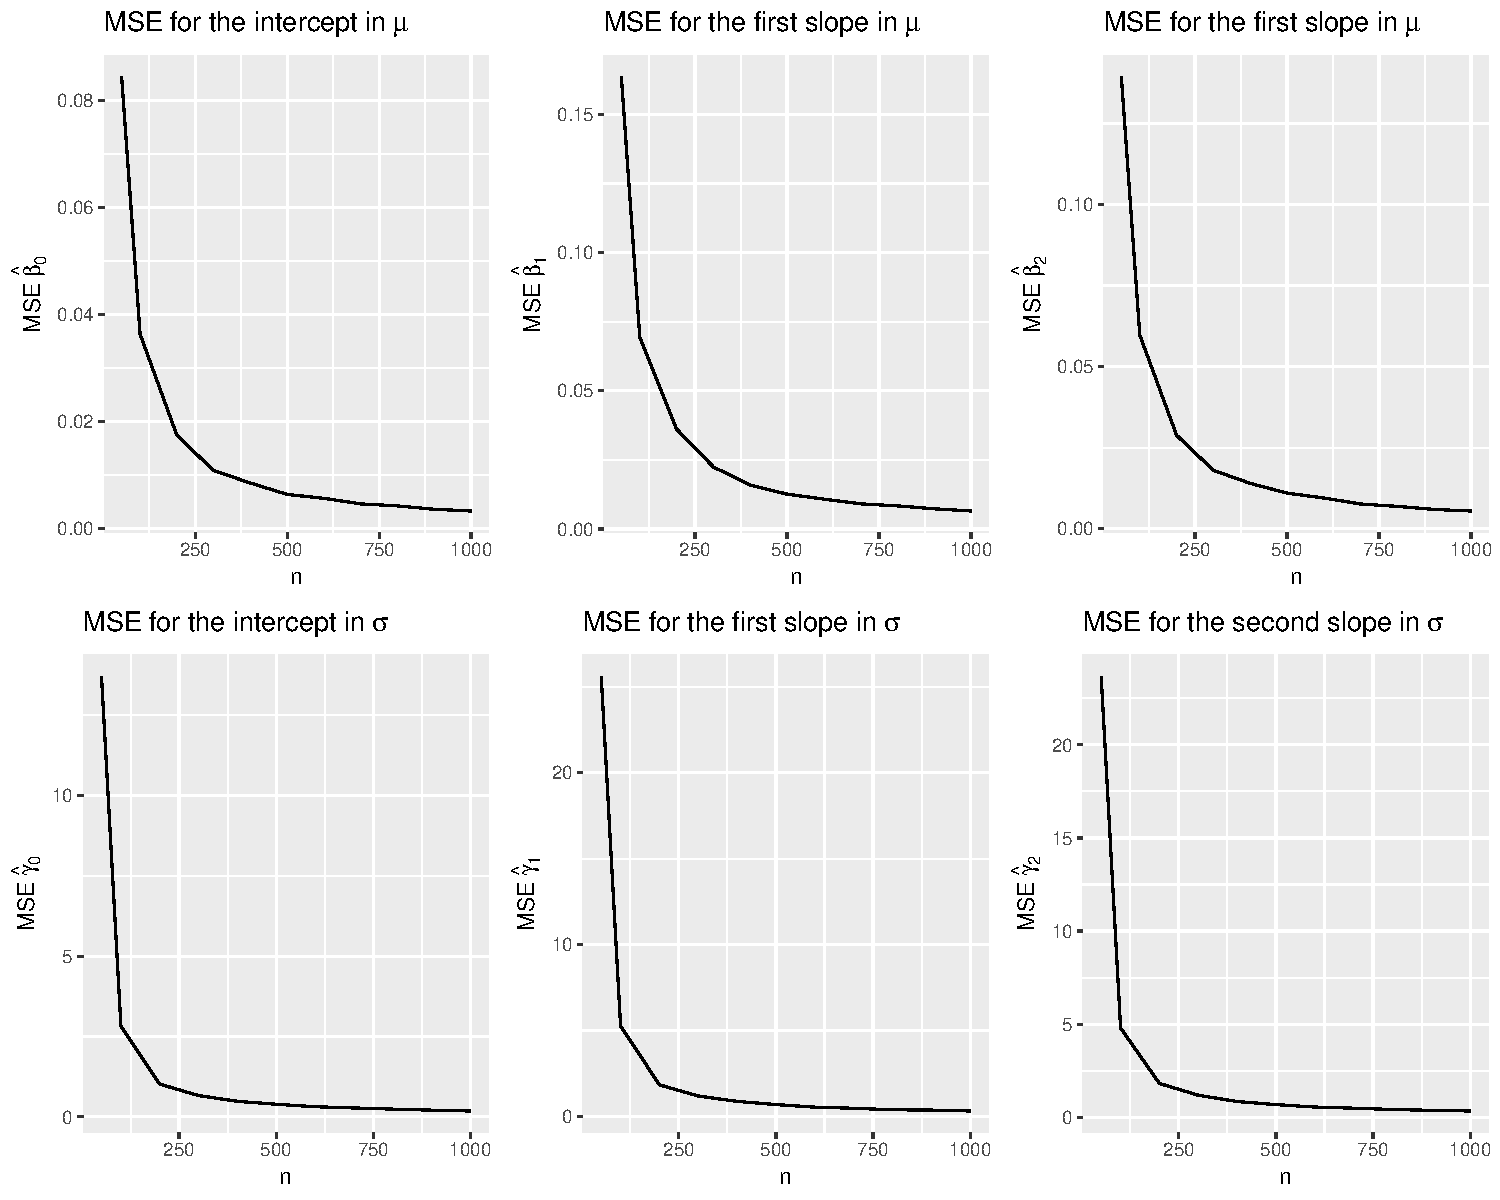
\includegraphics[width=0.6\linewidth,height=0.3\textheight,alt={}]{figures/case2_mse} 

}

\caption{Mean Squared Error for the estimated parameters $\hat{\beta}_0$, $\hat{\beta}_1$, $\hat{\beta}_2$, $\hat{\gamma}_0$, $\hat{\gamma}_1$ and $\hat{\gamma}_2$ versus $n$.}\label{fig:case2mse}
\end{figure}

\section{Application}\label{application}

This section presents the proposed regression model for analyzing the number of bids of some US firms. We consider data from \citet{cameron1997} and revisited by \citet{Saez13} regarding the number of bids received by 126 US firms that were targets of tender offers between 1978 and 1985. These firms were ultimately acquired within 52 weeks of the initial offer. The dependent variable of interest is the count of bids the target firm receives after the initial bid (\texttt{numbids}). The explanatory variables are:

\begin{itemize}
\tightlist
\item
  \texttt{leglrest}: equals 1 if legal defense by lawsuit.
\item
  \texttt{rearest}: equals 1 if proposed changes in asset structure.
\item
  \texttt{finrest}: equals 1 if proposed changes in ownership structure
\item
  \texttt{whtknght}: equals 1 if management invitation for friendly third-party bid.
\item
  \texttt{bidprem}: bid price divided by price 14 working days before bid.
\item
  \texttt{insthold}: percentage of stock held by institutions.
\item
  \texttt{size}: total book value of assets in billions of dollars.
\item
  \texttt{regulatn}: equals 1 if intervention by the federal regulator.
\end{itemize}

The dataset \texttt{Bids} is available in the \CRANpkg{Ecdat} R package by \citet{Ecdat_pack}. Figure \ref{fig:histnumberbids} depicts a barplot with the frequency for the response variable number of bids received by US firms. The mean and variance for the number of bids are 1.74 and 2.05, respectively. As the variance is slightly greater than the mean, this means that the data present overdispersion.

\begin{figure}

{\centering 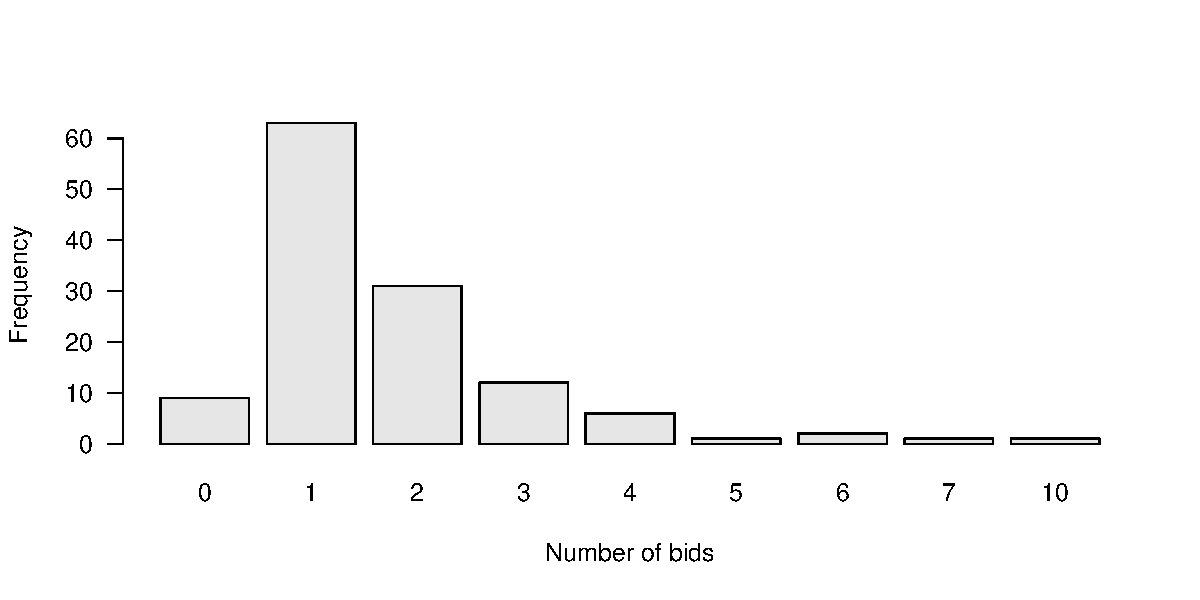
\includegraphics[width=0.6\linewidth,height=0.2\textheight,alt={}]{figures/hist_number_bids} 

}

\caption{Histogram for the number of bids received by US firms.}\label{fig:histnumberbids}
\end{figure}

In this illustration, we fitted the same model considered by \citet{Saez13} using the second parameterization for the hyper-Poisson distribution (HYPERPO2). The target model can be summarized as follows:

\begin{equation}
\begin{split}
numbids &\sim HYPERPO2(\mu, \sigma), \\
        \log(\mu) &=\beta_0 + \beta_1 \, leglrest + \beta_2 rearest + \beta_3 finrest + \beta_4 whtknght \\ 
     & \quad + \beta_5 bidprem + \beta_6 insthold + \beta_7 size + \beta_8 size^2 + \beta_9 regulatn ,  \\
\log(\sigma) &= \gamma_0 + \gamma_1 \, rearest + \gamma_2 finrest + \gamma_3 bidprem + \gamma_4 regulatn.
\end{split}
\label{eq:modbids01} 
\end{equation}

With the R code below, we can fit the model using the proposed functions in the \CRANpkg{DiscreteDists} R package \citep{DiscreteDists_pack}.

\begin{verbatim}
library(Ecdat)
library(DiscreteDists)
library(gamlss)
mod3 <- gamlss(numbids ~ leglrest + rearest + finrest + 
                         whtknght + bidprem + insthold + 
                         size + I(size^2) + regulatn,
               sigma.fo= ~ rearest + finrest + 
                           bidprem + regulatn,
               family=HYPERPO2, 
               data=Bids,
               control=gamlss.control(n.cyc=150, trace=TRUE))
\end{verbatim}

After adjusting the model, we obtain the parameter estimates shown in Table 3. This model has a \(BIC=386.48\) and pseudo \(R^2=0.47\), better values when compared to a classical Poisson model with \(BIC=418.25\) and pseudo \(R^2=0.23\).

\begin{table}[h]
\centering
\begin{tabular}{rrrrr} \hline
 \multicolumn{5}{c}{Estimated effects in modeling $\log(\mu)$}\\ \hline
 & Estimate & Std. Error & $t$-value & $P(>|t|)$ \\ \hline
Intercept & 1.8625 & 0.1390 & 13.3965 & 0.0000 \\ 
  leglrest & 0.2048 & 0.1215 & 1.6863 & 0.0946 \\ 
  rearest & -0.3489 & 0.1506 & -2.3159 & 0.0224 \\ 
  finrest & 0.4368 & 0.2098 & 2.0819 & 0.0397 \\ 
  whtknght & 0.3617 & 0.1078 & 3.3573 & 0.0011 \\ 
  bidprem & -1.1770 & 0.0928 & -12.6789 & 0.0000 \\ 
  insthold & -0.9665 & 0.1016 & -9.5084 & 0.0000 \\ 
  size & 0.1753 & 0.0344 & 5.0958 & 0.0000 \\ 
  $\text{size}^2$ & -0.0094 & 0.0022 & -4.2336 & 0.0000 \\ 
  regulatn & 0.2551 & 0.1386 & 1.8400 & 0.0684 \\ \hline
  \multicolumn{5}{c}{Estimated effects in modeling $\log(\sigma)$}\\ \hline
  Intercept & 31.1371 & 0.0944 & 329.9483 & 0.0000 \\ 
  rearest & 4.1331 & 1.1658 & 3.5452 & 0.0006 \\ 
  finrest & 9.9899 & 2.1817 & 4.5790 & 0.0000 \\ 
  bidprem & -29.2006 & 0.0908 & -321.6851 & 0.0000 \\ 
  regulatn & 6.3391 & 1.1863 & 5.3436 & 0.0000 \\ 
  \hline
\end{tabular}
\caption{Estimated effects for $\log(\mu)$ and $\log(\sigma)$ to model the Number of Bids using the model (17).}\label{table:res_numbids}
\end{table}

Figure \ref{fig:wormplot} shows the worm plot and the Randomized Quantile Residual (RQR) plot \citep{wormplot_2001}. From the worm plot, we can observe that the points and the red curve are inside the dashed curve lines, indicating that the fitted model explains the observed pattern for the response variable. Additionally, the RQR plot indicates no departure from the expected pattern from a Normal distribution for the Randomized Quantile Residuals.

\begin{figure}

{\centering 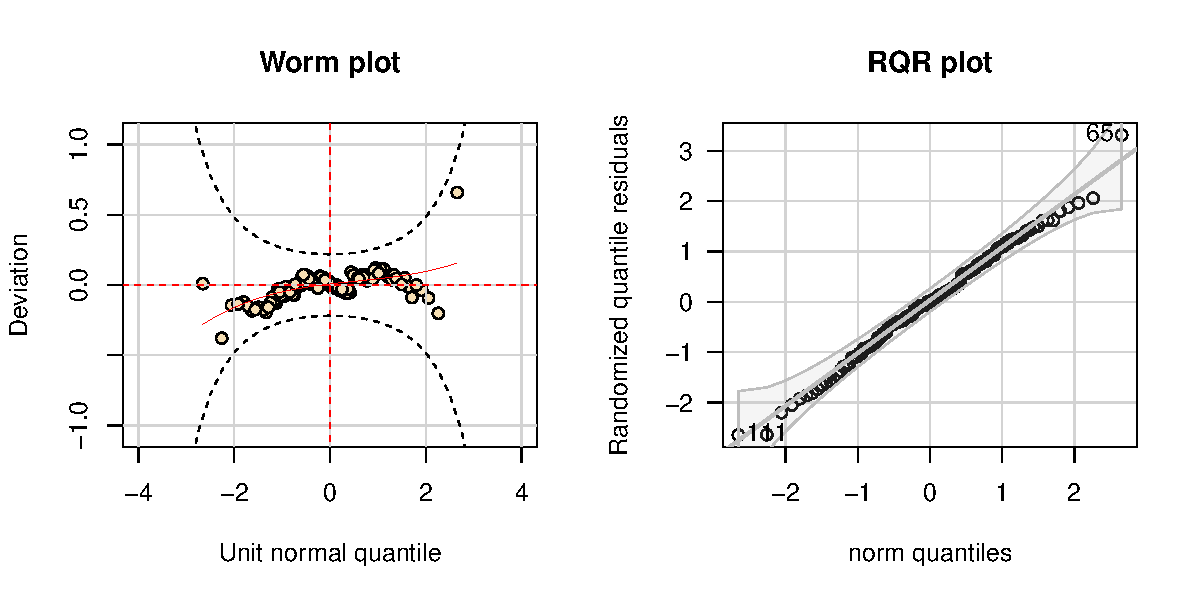
\includegraphics[width=0.6\linewidth,height=0.18\textheight,alt={}]{figures/worm_rqr_plot} 

}

\caption{Worm plot and RQR plot for Number of bids model with HYPERPO2 distribution.}\label{fig:wormplot}
\end{figure}

\section{Conclusions}\label{conclusions}

The hyper-Poisson regression model, which can handle both under-dispersed and over-dispersed data, is integrated into the Generalized Additive Models for Location, Scale, and Shape (GAMLSS) framework using the \CRANpkg{DiscreteDists} package. The new package addresses the shortcomings of the previously proposed \CRANpkg{DGLMExtPois} package, which lacks functions for computing probabilities, quantiles, and generating random values for the hyper-Poisson distribution. The \CRANpkg{DiscreteDists} package supports two parameterizations of the hyper-Poisson distribution which are: (i) \texttt{HYPERPO(mu,\ sigma)}, and (ii) \texttt{HYPERPO2(mu,\ sigma)}. The first parameterization is in line with the original proposal of \cite{BardwellCrow1964}, where the expected value \(E(Y)\) depends on both \(\mu\) and \(\sigma\). The second parameterization simplifies the \(E(Y)\) to equal \(\mu\), making it more appealing to users. The package provides functions for calculating probabilities, cumulative probabilities, quantiles, generating random samples, and estimating parameters within the GAMLSS framework for both parameterizations.

A Monte Carlo simulation study was carried out to assess the effectiveness of the estimators using their mean value and Mean Squared Error (MSE). First, data were generated from a \(HYPERPO(\mu, \sigma)\) distribution without covariates, where the parameters were estimated across various sample sizes. The results of the simulations have been discussed in the appropriate section (even with suitable plots), but in general, parameter estimates converged consistently to their true values as the sample sizes increased. In the second part of the study where data were generated from a model that included covariates, a similar trend was observed (i.e., larger sample sizes led to estimators that approached the true parameter values), and not surprisingly, in both situations, the Mean Squared Error (MSE) of estimates decreased monotonously towards zero. These results confidently attest to the utility and effectiveness of the \CRANpkg{DiscreteDists} package machinery in fitting the hyper-Poisson distribution model for datasets with/without covariates.

\bibliography{RJreferences.bib}

\address{%
Freddy Hernández-Barajas\\
Universidad Nacional de Colombia - sede Medellín\\%
Carrera 65 Nro. 59A - 110\\ Medellín, Colombia\\
%
\url{https://fhernanb.github.io/}\\%
\textit{ORCiD: \href{https://orcid.org/0000-0001-7459-3329}{0000-0001-7459-3329}}\\%
\href{mailto:fhernanb@unal.edu.co}{\nolinkurl{fhernanb@unal.edu.co}}%
}

\address{%
Jamiu S. Olumoh\\
American University of Nigeria\\%
Department of Mathematics and Statistics, Yola, 640001\\ Nigeria\\
%
%
\textit{ORCiD: \href{https://orcid.org/0000-0002-7371-3920}{0000-0002-7371-3920}}\\%
\href{mailto:jamiu.olumoh@aun.edu.ng}{\nolinkurl{jamiu.olumoh@aun.edu.ng}}%
}

\address{%
Osho O. Ajayi\\
American University of Nigeria\\%
Department of Mathematics and Statistics, Yola, 640001\\ Nigeria\\
%
%
\textit{ORCiD: \href{https://orcid.org/0000-0002-2436-3338}{0000-0002-2436-3338}}\\%
\href{mailto:osho.ajayi@aun.edu.ng}{\nolinkurl{osho.ajayi@aun.edu.ng}}%
}

\address{%
Fernando Marmolejo-Ramos\\
Flinders University\\%
Adelaide, 5042\\ Australia\\
%
%
\textit{ORCiD: \href{https://orcid.org/0000-0003-4680-1287}{0000-0003-4680-1287}}\\%
\href{mailto:fernando.marmolejoramos@flinders.edu.au}{\nolinkurl{fernando.marmolejoramos@flinders.edu.au}}%
}
